% Options for packages loaded elsewhere
\PassOptionsToPackage{unicode}{hyperref}
\PassOptionsToPackage{hyphens}{url}
%
\documentclass[
]{article}
\usepackage{amsmath,amssymb}
\usepackage{iftex}
\ifPDFTeX
  \usepackage[T1]{fontenc}
  \usepackage[utf8]{inputenc}
  \usepackage{textcomp} % provide euro and other symbols
\else % if luatex or xetex
  \usepackage{unicode-math} % this also loads fontspec
  \defaultfontfeatures{Scale=MatchLowercase}
  \defaultfontfeatures[\rmfamily]{Ligatures=TeX,Scale=1}
\fi
\usepackage{lmodern}
\ifPDFTeX\else
  % xetex/luatex font selection
\fi
% Use upquote if available, for straight quotes in verbatim environments
\IfFileExists{upquote.sty}{\usepackage{upquote}}{}
\IfFileExists{microtype.sty}{% use microtype if available
  \usepackage[]{microtype}
  \UseMicrotypeSet[protrusion]{basicmath} % disable protrusion for tt fonts
}{}
\makeatletter
\@ifundefined{KOMAClassName}{% if non-KOMA class
  \IfFileExists{parskip.sty}{%
    \usepackage{parskip}
  }{% else
    \setlength{\parindent}{0pt}
    \setlength{\parskip}{6pt plus 2pt minus 1pt}}
}{% if KOMA class
  \KOMAoptions{parskip=half}}
\makeatother
\usepackage{xcolor}
\usepackage[margin=1in]{geometry}
\usepackage{color}
\usepackage{fancyvrb}
\newcommand{\VerbBar}{|}
\newcommand{\VERB}{\Verb[commandchars=\\\{\}]}
\DefineVerbatimEnvironment{Highlighting}{Verbatim}{commandchars=\\\{\}}
% Add ',fontsize=\small' for more characters per line
\usepackage{framed}
\definecolor{shadecolor}{RGB}{248,248,248}
\newenvironment{Shaded}{\begin{snugshade}}{\end{snugshade}}
\newcommand{\AlertTok}[1]{\textcolor[rgb]{0.94,0.16,0.16}{#1}}
\newcommand{\AnnotationTok}[1]{\textcolor[rgb]{0.56,0.35,0.01}{\textbf{\textit{#1}}}}
\newcommand{\AttributeTok}[1]{\textcolor[rgb]{0.13,0.29,0.53}{#1}}
\newcommand{\BaseNTok}[1]{\textcolor[rgb]{0.00,0.00,0.81}{#1}}
\newcommand{\BuiltInTok}[1]{#1}
\newcommand{\CharTok}[1]{\textcolor[rgb]{0.31,0.60,0.02}{#1}}
\newcommand{\CommentTok}[1]{\textcolor[rgb]{0.56,0.35,0.01}{\textit{#1}}}
\newcommand{\CommentVarTok}[1]{\textcolor[rgb]{0.56,0.35,0.01}{\textbf{\textit{#1}}}}
\newcommand{\ConstantTok}[1]{\textcolor[rgb]{0.56,0.35,0.01}{#1}}
\newcommand{\ControlFlowTok}[1]{\textcolor[rgb]{0.13,0.29,0.53}{\textbf{#1}}}
\newcommand{\DataTypeTok}[1]{\textcolor[rgb]{0.13,0.29,0.53}{#1}}
\newcommand{\DecValTok}[1]{\textcolor[rgb]{0.00,0.00,0.81}{#1}}
\newcommand{\DocumentationTok}[1]{\textcolor[rgb]{0.56,0.35,0.01}{\textbf{\textit{#1}}}}
\newcommand{\ErrorTok}[1]{\textcolor[rgb]{0.64,0.00,0.00}{\textbf{#1}}}
\newcommand{\ExtensionTok}[1]{#1}
\newcommand{\FloatTok}[1]{\textcolor[rgb]{0.00,0.00,0.81}{#1}}
\newcommand{\FunctionTok}[1]{\textcolor[rgb]{0.13,0.29,0.53}{\textbf{#1}}}
\newcommand{\ImportTok}[1]{#1}
\newcommand{\InformationTok}[1]{\textcolor[rgb]{0.56,0.35,0.01}{\textbf{\textit{#1}}}}
\newcommand{\KeywordTok}[1]{\textcolor[rgb]{0.13,0.29,0.53}{\textbf{#1}}}
\newcommand{\NormalTok}[1]{#1}
\newcommand{\OperatorTok}[1]{\textcolor[rgb]{0.81,0.36,0.00}{\textbf{#1}}}
\newcommand{\OtherTok}[1]{\textcolor[rgb]{0.56,0.35,0.01}{#1}}
\newcommand{\PreprocessorTok}[1]{\textcolor[rgb]{0.56,0.35,0.01}{\textit{#1}}}
\newcommand{\RegionMarkerTok}[1]{#1}
\newcommand{\SpecialCharTok}[1]{\textcolor[rgb]{0.81,0.36,0.00}{\textbf{#1}}}
\newcommand{\SpecialStringTok}[1]{\textcolor[rgb]{0.31,0.60,0.02}{#1}}
\newcommand{\StringTok}[1]{\textcolor[rgb]{0.31,0.60,0.02}{#1}}
\newcommand{\VariableTok}[1]{\textcolor[rgb]{0.00,0.00,0.00}{#1}}
\newcommand{\VerbatimStringTok}[1]{\textcolor[rgb]{0.31,0.60,0.02}{#1}}
\newcommand{\WarningTok}[1]{\textcolor[rgb]{0.56,0.35,0.01}{\textbf{\textit{#1}}}}
\usepackage{longtable,booktabs,array}
\usepackage{calc} % for calculating minipage widths
% Correct order of tables after \paragraph or \subparagraph
\usepackage{etoolbox}
\makeatletter
\patchcmd\longtable{\par}{\if@noskipsec\mbox{}\fi\par}{}{}
\makeatother
% Allow footnotes in longtable head/foot
\IfFileExists{footnotehyper.sty}{\usepackage{footnotehyper}}{\usepackage{footnote}}
\makesavenoteenv{longtable}
\usepackage{graphicx}
\makeatletter
\def\maxwidth{\ifdim\Gin@nat@width>\linewidth\linewidth\else\Gin@nat@width\fi}
\def\maxheight{\ifdim\Gin@nat@height>\textheight\textheight\else\Gin@nat@height\fi}
\makeatother
% Scale images if necessary, so that they will not overflow the page
% margins by default, and it is still possible to overwrite the defaults
% using explicit options in \includegraphics[width, height, ...]{}
\setkeys{Gin}{width=\maxwidth,height=\maxheight,keepaspectratio}
% Set default figure placement to htbp
\makeatletter
\def\fps@figure{htbp}
\makeatother
\setlength{\emergencystretch}{3em} % prevent overfull lines
\providecommand{\tightlist}{%
  \setlength{\itemsep}{0pt}\setlength{\parskip}{0pt}}
\setcounter{secnumdepth}{-\maxdimen} % remove section numbering
\usepackage{booktabs}
\usepackage{longtable}
\usepackage{array}
\usepackage{multirow}
\usepackage{wrapfig}
\usepackage{float}
\usepackage{colortbl}
\usepackage{pdflscape}
\usepackage{tabu}
\usepackage{threeparttable}
\usepackage{threeparttablex}
\usepackage[normalem]{ulem}
\usepackage{makecell}
\usepackage{xcolor}
\ifLuaTeX
  \usepackage{selnolig}  % disable illegal ligatures
\fi
\IfFileExists{bookmark.sty}{\usepackage{bookmark}}{\usepackage{hyperref}}
\IfFileExists{xurl.sty}{\usepackage{xurl}}{} % add URL line breaks if available
\urlstyle{same}
\hypersetup{
  pdftitle={Lab 4: Matrix population models},
  pdfauthor={NRES 470/670},
  hidelinks,
  pdfcreator={LaTeX via pandoc}}

\title{Lab 4: Matrix population models}
\author{NRES 470/670}
\date{Spring 2024}

\begin{document}
\maketitle

In this lab we will continue to work with age-structured populations:
specifically, we will get familiar with \textbf{matrix projection
models}! Remember that while matrix population models may look
complicated, they are just a modified version of the \emph{discrete}
exponential growth model: \(N_{t+1}=\lambda \cdot N_t\).

If you want to follow along in R, you can find the R script
\href{LAB4.R}{here}. I recommend right-clicking on the link, saving the
script to a designated folder, and loading up the script in RStudio.

\hypertarget{mathematics-of-matrix-population-models}{%
\subsection{Mathematics of matrix population
models:}\label{mathematics-of-matrix-population-models}}

We all remember the discrete population growth equation:

\(N_{t+1}=\lambda \cdot N_t \qquad \text{(Eq. 1)}\),

where \(N\) represents abundance (as always), \(t\) is time (often in
years), and \(\lambda\) is the multiplicative growth rate over the time
period \(t \rightarrow t+1\)

In other words, \(\lambda\) is the number you multiply this years
abundance by to compute next year's abundance.

The matrix population growth equation looks pretty much the same!

\(\mathbf{N}_{t+1} = \mathbf{A} \cdot \mathbf{N}_{t} \qquad \text{(Eq. 2)}\),

where \(\mathbf{N}\) is a \textbf{vector} of abundances (a `package' of
numbers representing abundances for each life stage), and \(\mathbf{A}\)
is the \textbf{transition matrix} (a `package' of numbers representing
per-capita transition rates among life stages from one year to the
next).

We can be more explicit about this if we re-write the above equation
this way:

\(\begin{bmatrix}N_1\\ N_2\\N_3 \end{bmatrix}_{t+1}=\begin{bmatrix}F_1 & F_2 & F_3\\ P_{1 \rightarrow 2} & P_{2 \rightarrow 2} & 0\\ 0 & P_{2 \rightarrow 3} & P_{3 \rightarrow 3}\end{bmatrix} \cdot \begin{bmatrix}N_1\\ N_2\\N_3 \end{bmatrix}_{t} \qquad \text{(Eq. 3)}\)

Where \(P_{1 \rightarrow 2}\) is the probability of advancing from Stage
1 to Stage 2 (fraction of Stage 1 individuals that survive and
transition to Stage 2), and \(F_2\) is the \textbf{fecundity} of stage 2
(per-capita offspring production by individuals that started the year in
Stage 2).

\hypertarget{the-transition-matrix}{%
\subsubsection{The Transition Matrix}\label{the-transition-matrix}}

The transition matrix must be a \emph{square matrix} -- meaning that the
number of rows is the same as the number of columns. There must be the
same number of rows and columns as there are life stages for the species
you are modeling. If there are 5 life stages, your transition matrix
must have five rows and five columns.

\hypertarget{age-structured-model-leslie-matrix}{%
\paragraph{Age structured model (Leslie
matrix)}\label{age-structured-model-leslie-matrix}}

The term `\textbf{Leslie Matrix}' refers to a specific type of matrix
population model where each stage represents one year of life (this is
an \textbf{age-structured} model.

In this class, we will assume that the first age class represents
one-year-olds, and that the first row of a transition matrix (i.e., the
``fecundity row'') represents the entry of new one-year-olds into the
population.

In a Leslie matrix, no individuals can ever stay the same age for more
than one year (obviously). So, terms like \(P_{2 \rightarrow 2}\), or
\(P_{3 \rightarrow 3}\) must be set to zero by definition.

Each age class is associated with only one survival rate, and this rate
involves transitioning to the next age (one year older!). That is,
survival is represented by only one term per age: e.g.,
\(P_{2 \rightarrow 3}\), or \(P_{3 \rightarrow 4}\)

For a Leslie matrix, the final year of life must have a survival rate of
zero. Why? Because no individual can survive past the final year of
life!

In this class, we will \emph{always} assume that reproduction occurs at
the very beginning of each time step. This type of matrix model is known
as a ``pre-breeding census'' because we assume that breeding takes place
right after we monitor our population. In this way, the youngest age we
ever observe are individuals that were born right after last year's
survey- meaning, one-year-olds!

This means that all \textbf{fecundity} terms in our transition matrices
must be computed as the product of birth rate and survival through the
first year of life (i.e., all newborns from this year must survive for a
full year before they can ``enter'' the study as one-year-olds in the
following year)

In a Leslie Matrix (pre-breeding census version), the term \(F_1\) must
be computed as the per-capita birth rate associated with one-year-olds,
\(b(1)\), multiplied by the probability of their offspring surviving
through the first year of life, \(P_{0 \rightarrow 1}\):

\(F_1=b(1) \cdot P_{0 \rightarrow 1}\)

Similarly,

\(F_2=b(2) \cdot P_{0 \rightarrow 1}\)\\
\(F_3=b(3) \cdot P_{0 \rightarrow 1}\)

Here's an example of an age-structured (Leslie) matrix:

\(\begin{bmatrix}N_1\\N_2\\ N3 \end{bmatrix}_{t+1}=\begin{bmatrix}F_1 & F_2 & F_3\\ P_{1 \rightarrow 2} & 0 & 0\\ 0 & P_{2 \rightarrow 3} & 0\end{bmatrix} \cdot \begin{bmatrix}N_1\\N_2\\N3 \end{bmatrix}_{t} \qquad \text{(Eq. 3)}\)

\hypertarget{stage-structured-model-lefkovitch-matrix}{%
\paragraph{Stage structured model (Lefkovitch
matrix)}\label{stage-structured-model-lefkovitch-matrix}}

When a matrix is used to represent a stage-structured population, it is
often called a 'Lefkovitch'' (or stage-based) matrix.

NOTE: \emph{survival \emph{P} in a stage-structured transition matrix is
NOT necessarily the same thing as survival rate} (e.g., g(x) from a life
table). What's the difference? The answer is that survivors from one age
class may end up in more than one class. For example, some fraction of
Stage 2 individuals may survive but remain in Stage 2 next year
(\(P_{2 \rightarrow 2}\)). Another subset of survivors may end up in
Stage 3 (\(P_{2 \rightarrow 3}\)). Together, these two rates (added
together) represent the total survival of Stage 2 individuals!

In contrast: in a Leslie matrix, all individuals must either transition
to the next stage or die. Always remember that (just like in a Leslie
matrix) \emph{fecundity \emph{F} in a stage transition matrix is NOT the
same thing as the age-specific per-capita birth rates \emph{b(x)}} from
a life table.

Instead, the Fecundity terms in a stage-transition matrix \(F_{S}\) also
takes into account the \emph{survival rate} of the offspring (e.g.,
\(P_{S0 \rightarrow S1}\))!! For an adult of stage \(S\) to contribute
to the next generation, \emph{it must first give birth and their
offspring must survive their first year of life}!.

\(F_S = b(this \space year) \cdot P_{first \space year \space of \space life} \qquad \text{(Eq. 4)}\)

Computation of fecundity can get fairly complicated, but if you start to
get confused, always return to this basic principle: \emph{fecundity is
birth rate times first-year survival}.

\(F_1=b(1) \cdot P_{0 \rightarrow 1}\)\\
\(F_2=b(2) \cdot P_{0 \rightarrow 1}\)\\
\(F_3=b(3) \cdot P_{0 \rightarrow 1}\)

\hypertarget{matrix-operations}{%
\subsubsection{Matrix operations:}\label{matrix-operations}}

There is a lot we can do with matrix population models. The most obvious
one is \emph{projection}:

\hypertarget{projection}{%
\paragraph{Projection:}\label{projection}}

This lab demo contains a bunch of R code (R makes it pretty easy - and
fast- to run matrix population models!).

If you want to follow along in R, you can find the R script
\href{LAB4.R}{here}.

We have already seen the matrix projection equation (Eq. 2, above). Here
is how we can implement this in R:

\begin{Shaded}
\begin{Highlighting}[]
\CommentTok{\# Matrix projection in R {-}{-}{-}{-}{-}{-}{-}{-}{-}{-}{-}{-}{-}{-}{-}{-}{-}{-}{-}{-}{-}}

\CommentTok{\# Syntax for projecting abundance using a transition matrix (}\AlertTok{NOTE}\CommentTok{: this code won\textquotesingle{}t run until we specify the terms on the right)}

\CommentTok{\# Year1 \textless{}{-} projection\_matrix \%*\% Abundance\_year0  \# matrix multiplication!}
\end{Highlighting}
\end{Shaded}

Let's try it:

First, build a projection matrix:

\begin{Shaded}
\begin{Highlighting}[]
\CommentTok{\# First, build a simple projection matrix called TMat}

\NormalTok{TMat }\OtherTok{\textless{}{-}} \FunctionTok{matrix}\NormalTok{(     }\CommentTok{\# }
  \FunctionTok{c}\NormalTok{(}
    \FloatTok{0.25}\NormalTok{,     }\FloatTok{1.5}\NormalTok{,   }\FloatTok{1.5}\NormalTok{,}
    \FloatTok{0.4}\NormalTok{,   }\DecValTok{0}\NormalTok{,     }\DecValTok{0}\NormalTok{,}
    \DecValTok{0}\NormalTok{,     }\FloatTok{0.75}\NormalTok{,   }\DecValTok{0}
\NormalTok{  )}
\NormalTok{  ,}\AttributeTok{nrow=}\DecValTok{3}\NormalTok{,}\AttributeTok{ncol=}\DecValTok{3}\NormalTok{,}\AttributeTok{byrow=}\NormalTok{T}
\NormalTok{)}
\NormalTok{TMat    }\CommentTok{\# print to the console to check!}
\end{Highlighting}
\end{Shaded}

\begin{verbatim}
##      [,1] [,2] [,3]
## [1,] 0.25 1.50  1.5
## [2,] 0.40 0.00  0.0
## [3,] 0.00 0.75  0.0
\end{verbatim}

\textbf{Q}: is this an age-structured (Leslie) or stage-structured
(Lefkovitch) matrix?

Next, let's build an initial abundance vector:

\begin{Shaded}
\begin{Highlighting}[]
\CommentTok{\# Then we specify initial abundances for the three age classes}

\NormalTok{InitAbund }\OtherTok{\textless{}{-}} \FunctionTok{c}\NormalTok{(}\DecValTok{1000}\NormalTok{,}\DecValTok{0}\NormalTok{,}\DecValTok{0}\NormalTok{)    }\CommentTok{\# initial abundance vector}
\NormalTok{InitAbund    }\CommentTok{\# print to the console to check!}
\end{Highlighting}
\end{Shaded}

\begin{verbatim}
## [1] 1000    0    0
\end{verbatim}

Now we can run our first projection- this time, we will use the
transition matrix to compute the abundance vector for year 1!

\begin{Shaded}
\begin{Highlighting}[]
\CommentTok{\# Now we can run the code for real}

\CommentTok{\# project year{-}1 abundance:}

\NormalTok{Year1 }\OtherTok{\textless{}{-}}\NormalTok{ TMat }\SpecialCharTok{\%*\%}\NormalTok{ InitAbund  }\CommentTok{\# matrix multiplication in R uses the symbol \textquotesingle{}\%*\%\textquotesingle{}}
\NormalTok{Year1}
\end{Highlighting}
\end{Shaded}

\begin{verbatim}
##      [,1]
## [1,]  250
## [2,]  400
## [3,]    0
\end{verbatim}

Now we have 400 individuals in stage 2!

Let's project one more year:

\begin{Shaded}
\begin{Highlighting}[]
\CommentTok{\# Project year{-}2 abundance}

\NormalTok{Year2 }\OtherTok{\textless{}{-}}\NormalTok{ TMat }\SpecialCharTok{\%*\%}\NormalTok{ Year1  }\CommentTok{\# matrix multiplication!}
\NormalTok{Year2}
\end{Highlighting}
\end{Shaded}

\begin{verbatim}
##       [,1]
## [1,] 662.5
## [2,] 100.0
## [3,] 300.0
\end{verbatim}

Finally, here is some code to project many years into the future! You
may want to re-use some of this code for the exercises below.

\begin{Shaded}
\begin{Highlighting}[]
\CommentTok{\# Multi{-}year projection code {-}{-}{-}{-}{-}{-}{-}{-}{-}{-}{-}{-}{-}{-}{-}{-}{-}{-}{-}{-}{-}{-}{-}{-}{-}{-}{-}{-}}

\CommentTok{\#  You may want to modify this code for the examples below:}


\CommentTok{\# Set key parameters {-}{-}{-}{-}{-}{-}{-}{-}{-}{-}{-}{-}{-}{-}{-}{-}{-}{-}{-}{-}{-}{-}{-}}

\NormalTok{nYears }\OtherTok{\textless{}{-}} \DecValTok{20}                                            \CommentTok{\# set the number of years to project}
\NormalTok{TMat }\OtherTok{\textless{}{-}} \FunctionTok{matrix}\NormalTok{(     }\CommentTok{\# }
  \FunctionTok{c}\NormalTok{(}
    \FloatTok{0.25}\NormalTok{,     }\FloatTok{1.5}\NormalTok{,   }\FloatTok{1.5}\NormalTok{,}
    \FloatTok{0.4}\NormalTok{,   }\DecValTok{0}\NormalTok{,     }\DecValTok{0}\NormalTok{,}
    \DecValTok{0}\NormalTok{,     }\FloatTok{0.75}\NormalTok{,   }\DecValTok{0}
\NormalTok{  )}
\NormalTok{  ,}\AttributeTok{nrow=}\DecValTok{3}\NormalTok{,}\AttributeTok{ncol=}\DecValTok{3}\NormalTok{,}\AttributeTok{byrow=}\NormalTok{T}
\NormalTok{)}
\NormalTok{InitAbund }\OtherTok{\textless{}{-}} \FunctionTok{c}\NormalTok{(}\DecValTok{1000}\NormalTok{,}\DecValTok{0}\NormalTok{,}\DecValTok{0}\NormalTok{)                                }\CommentTok{\# initial abundance vector}
\NormalTok{AgeStructured }\OtherTok{\textless{}{-}} \ConstantTok{TRUE}          \CommentTok{\# set to TRUE for Leslie matrix and FALSE for Lefkovitch }


\CommentTok{\# Use a FOR loop for multi{-}year projection  {-}{-}{-}{-}{-}{-}{-}{-}{-}{-}{-}{-}{-}}

   \CommentTok{\# }\AlertTok{NOTE}\CommentTok{: the code below can be re{-}used without modification:}

\NormalTok{allYears }\OtherTok{\textless{}{-}} \FunctionTok{matrix}\NormalTok{(}\DecValTok{0}\NormalTok{,}\AttributeTok{nrow=}\FunctionTok{nrow}\NormalTok{(TMat),}\AttributeTok{ncol=}\NormalTok{nYears}\SpecialCharTok{+}\DecValTok{1}\NormalTok{)     }\CommentTok{\# build a storage array for all stages and all years!}
\NormalTok{allYears[,}\DecValTok{1}\NormalTok{] }\OtherTok{\textless{}{-}}\NormalTok{ InitAbund  }\CommentTok{\# set the year 0 abundance                                    }
\ControlFlowTok{for}\NormalTok{(t }\ControlFlowTok{in} \DecValTok{2}\SpecialCharTok{:}\NormalTok{(nYears}\SpecialCharTok{+}\DecValTok{1}\NormalTok{))\{   }\CommentTok{\# loop through all years}
\NormalTok{  allYears[,t] }\OtherTok{\textless{}{-}}\NormalTok{  TMat }\SpecialCharTok{\%*\%}\NormalTok{ allYears[,t}\DecValTok{{-}1}\NormalTok{]}
\NormalTok{\}}
\FunctionTok{plot}\NormalTok{(}\DecValTok{1}\NormalTok{,}\DecValTok{1}\NormalTok{,}\AttributeTok{pch=}\StringTok{""}\NormalTok{,}\AttributeTok{ylim=}\FunctionTok{c}\NormalTok{(}\DecValTok{0}\NormalTok{,}\FunctionTok{max}\NormalTok{(allYears)),}\AttributeTok{xlim=}\FunctionTok{c}\NormalTok{(}\DecValTok{0}\NormalTok{,nYears}\SpecialCharTok{+}\DecValTok{1}\NormalTok{),}\AttributeTok{xlab=}\StringTok{"Years"}\NormalTok{,}\AttributeTok{ylab=}\StringTok{"Abundance"}\NormalTok{,}\AttributeTok{xaxt=}\StringTok{"n"}\NormalTok{)  }\CommentTok{\# set up blank plot}
\NormalTok{cols }\OtherTok{\textless{}{-}} \FunctionTok{rainbow}\NormalTok{(}\FunctionTok{ncol}\NormalTok{(TMat))    }\CommentTok{\# set up colors to use}
\ControlFlowTok{for}\NormalTok{(s }\ControlFlowTok{in} \DecValTok{1}\SpecialCharTok{:}\FunctionTok{ncol}\NormalTok{(TMat))\{}
  \FunctionTok{points}\NormalTok{(allYears[s,],}\AttributeTok{col=}\NormalTok{cols[s],}\AttributeTok{type=}\StringTok{"l"}\NormalTok{,}\AttributeTok{lwd=}\DecValTok{2}\NormalTok{)     }\CommentTok{\# plot out each life stage abundance, one at a time}
\NormalTok{\}}
\FunctionTok{axis}\NormalTok{(}\DecValTok{1}\NormalTok{,}\AttributeTok{at=}\FunctionTok{seq}\NormalTok{(}\DecValTok{1}\NormalTok{,nYears}\SpecialCharTok{+}\DecValTok{1}\NormalTok{),}\AttributeTok{labels =} \FunctionTok{seq}\NormalTok{(}\DecValTok{0}\NormalTok{,nYears))   }\CommentTok{\# label the axis}
\ControlFlowTok{if}\NormalTok{(AgeStructured)\{}
\NormalTok{  leg }\OtherTok{\textless{}{-}}  \FunctionTok{paste}\NormalTok{(}\StringTok{"Age"}\NormalTok{,}\FunctionTok{seq}\NormalTok{(}\DecValTok{1}\NormalTok{,(}\FunctionTok{ncol}\NormalTok{(TMat))))}
\NormalTok{\}}\ControlFlowTok{else}\NormalTok{\{}
\NormalTok{  leg }\OtherTok{\textless{}{-}} \FunctionTok{paste}\NormalTok{(}\StringTok{"Stage"}\NormalTok{,}\FunctionTok{seq}\NormalTok{(}\DecValTok{1}\NormalTok{,}\FunctionTok{ncol}\NormalTok{(TMat))) }
\NormalTok{\}}
\FunctionTok{legend}\NormalTok{(}\StringTok{"topleft"}\NormalTok{,}\AttributeTok{col=}\NormalTok{cols,}\AttributeTok{lwd=}\FunctionTok{rep}\NormalTok{(}\DecValTok{2}\NormalTok{,}\FunctionTok{ncol}\NormalTok{(TMat)),}\AttributeTok{legend=}\NormalTok{leg,}\AttributeTok{bty=}\StringTok{"n"}\NormalTok{)  }\CommentTok{\# put a legend on the plot}
\end{Highlighting}
\end{Shaded}

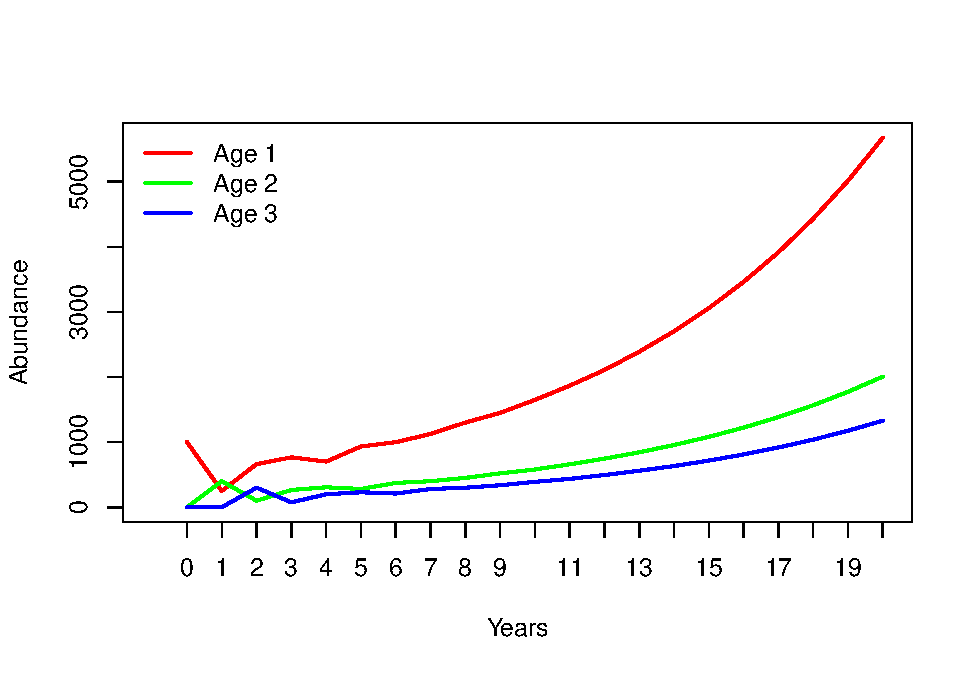
\includegraphics{LAB4_files/figure-latex/unnamed-chunk-10-1.pdf}

\hypertarget{compute-lambda}{%
\paragraph{Compute lambda}\label{compute-lambda}}

Clearly this is a growing population. But let's see exactly what
\(\lambda\) is!

NOTE: we are using a ``package'' in R to make these analyses super easy!
So if you don't already have the ``popbio'' package, go to the
``Packages'' tab in Rstudio (should be at the top of the lower right
panel), click on ``Install'', and then type ``popbio'' in the
``Packages'' field in the pop-up window, then click on the ``Install''
button.

\begin{Shaded}
\begin{Highlighting}[]
\CommentTok{\# Use \textquotesingle{}popbio\textquotesingle{} package to compute lambda and SSD {-}{-}{-}{-}{-}{-}{-}{-}{-}{-}{-}}

\CommentTok{\# Use the following line of code if you haven\textquotesingle{}t installed \textquotesingle{}popbio\textquotesingle{} yet. Once you\textquotesingle{}ve installed it, you can delete the line or comment this line out by adding a pound sign before the "i" in "install.packages"}

\CommentTok{\# install.packages("popbio")   \# uncomment this line to run {-} you only need to do this once}

\CommentTok{\# Use the \textquotesingle{}popbio\textquotesingle{} package to compute lambda (}\AlertTok{NOTE}\CommentTok{: you first have to install the popbio package! You only have to install the package once...)}

\FunctionTok{library}\NormalTok{(popbio)   }\CommentTok{\# load the \textquotesingle{}popbio\textquotesingle{} package in R}

\FunctionTok{lambda}\NormalTok{(TMat)}
\end{Highlighting}
\end{Shaded}

\begin{verbatim}
## [1] 1.13162
\end{verbatim}

Pretty easy!

\hypertarget{compute-stable-stage-distribution-s.s.d.}{%
\paragraph{Compute stable stage distribution
(S.S.D.)}\label{compute-stable-stage-distribution-s.s.d.}}

Clearly the population doesn't reach a stable stage distribution until a
few years into our simulation. What exactly is the stable stage
distribution here? We can do this in R:

\begin{Shaded}
\begin{Highlighting}[]
\CommentTok{\# Use the \textquotesingle{}popbio\textquotesingle{} package to compute the stable stage distribution!}

\FunctionTok{stable.stage}\NormalTok{(TMat)}
\end{Highlighting}
\end{Shaded}

\begin{verbatim}
## [1] 0.6298233 0.2226270 0.1475497
\end{verbatim}

Let's get started with running some matrix-based population models!

\hypertarget{exercise-1-age-structured-leslie-matrix-projection-models}{%
\subsection{Exercise 1: age-structured (Leslie) matrix projection
models!}\label{exercise-1-age-structured-leslie-matrix-projection-models}}

In this exercise, you will have a chance to play around with an
age-structured (Leslie) matrix population model. But first, you are
asked to translate a life table into an age-structured transition
matrix!

Here is the life table: \href{life_table4.xlsx}{Excel format}\\
\href{life_table4.csv}{CSV format}

\begin{longtable}[]{@{}rrr@{}}
\toprule\noalign{}
x & S(x) & b(x) \\
\midrule\noalign{}
\endhead
\bottomrule\noalign{}
\endlastfoot
0 & 1000 & 0.0 \\
1 & 350 & 0.0 \\
2 & 145 & 3.9 \\
3 & 70 & 4.2 \\
4 & 19 & 0.8 \\
5 & 0 & 0.0 \\
\end{longtable}

Translate the above \emph{life table} into an age-structured (Leslie)
transition matrix with four ages: age 1 (yearlings), age 2, age 3, and
age 4. You don't need to include age 5 because no individuals ever make
it past age 4.

Keep the following points in mind:

\begin{itemize}
\tightlist
\item
  There is no ``age 0'' (newborn) stage (since this is a ``pre-breeding
  census'' model). Individuals only ``enter'' the model if they are born
  and survive to age 1.
\item
  Individuals are in the ``age 1'' stage if they are between the ages of
  1 and 2 (that is, they are one-year-olds!). They transition to the
  ``age 2'' stage (\(P_{1 \rightarrow 2}\)) if they survive to age 2.\\
\item
  For individuals of the ``age 1'' class to contribute new offspring to
  the population in the next time step (\(F_0\)), they have to produce
  offspring when they are exactly 1 year of age (which they do at the
  rate of \(b(1)\) -- the birth rate at age 1), and their offspring must
  survive their first year of life (\(P_{0 \rightarrow 1}\)).\\
\item
  Use four age classes for your transition matrix (age 1 through 4).
  Individuals in the final age class (age 4) have zero survival (you
  can't survive to age 5) but a non-zero fecundity (four-year-olds can
  give birth, and their offspring can survive to become one-year-olds
  next year)\\
\item
  No individual ever stays the same age - they either transition to the
  next age or they die (this is how a \textbf{Leslie Matrix} model
  works).
\end{itemize}

NOTE: Gotelli uses the term `age class 1' to refer to individuals in
their first year of life (0-year-olds) and `age class 2' for individuals
in their second year of life (one-year-olds), but I think it's easier to
think of this as age 0, age 1, etc. That way, our age classes will match
the way we usually talk about age in years!

1a (image upload). Upload an image file of the full transition matrix
(16 numbers, arranged in 4 rows and 4 columns) to WebCampus. To maximize
your chance for partial credit, include all calculations you needed to
arrive at your final solution.

1b (short answer). Describe (in words) how you computed the number in
row 1, column 3 of your matrix (fecundity of 3-year-olds).

You will need to use R for the next few questions. Make sure you have
the `popbio' package installed in your R session!

You will need to enter your matrix from 1a into R, using something like
the following:

\begin{Shaded}
\begin{Highlighting}[]
\CommentTok{\# Construct a four{-}age matrix:}

\NormalTok{TMat }\OtherTok{\textless{}{-}} \FunctionTok{matrix}\NormalTok{(     }\CommentTok{\# }
  \FunctionTok{c}\NormalTok{(}
    \DecValTok{0}\NormalTok{,     }\FloatTok{1.9}\NormalTok{,   }\FloatTok{1.1}\NormalTok{,    }\FloatTok{0.4}\NormalTok{,   }
    \FloatTok{0.4}\NormalTok{,     }\DecValTok{0}\NormalTok{,     }\DecValTok{0}\NormalTok{,      }\DecValTok{0}\NormalTok{,    }
    \DecValTok{0}\NormalTok{,       }\FloatTok{0.75}\NormalTok{,  }\DecValTok{0}\NormalTok{,      }\DecValTok{0}\NormalTok{,   }
    \DecValTok{0}\NormalTok{,       }\DecValTok{0}\NormalTok{,     }\FloatTok{0.65}\NormalTok{,   }\DecValTok{0}  
\NormalTok{  )}
\NormalTok{  ,}\AttributeTok{nrow=}\DecValTok{4}\NormalTok{,}\AttributeTok{ncol=}\DecValTok{4}\NormalTok{,}\AttributeTok{byrow=}\NormalTok{T}
\NormalTok{)}
\NormalTok{TMat}
\end{Highlighting}
\end{Shaded}

\begin{verbatim}
##      [,1] [,2] [,3] [,4]
## [1,]  0.0 1.90 1.10  0.4
## [2,]  0.4 0.00 0.00  0.0
## [3,]  0.0 0.75 0.00  0.0
## [4,]  0.0 0.00 0.65  0.0
\end{verbatim}

1c (short answer- one number). What is the finite rate of growth
\(\lambda\) for this population? (HINT: use the `lambda()' function from
the popbio package)

1d (short answer). Based on this result, is this a growing population? A
declining population?

1e (short answer- 4 numbers). What is the stable-stage distribution
(SSD) for this population (fraction of the population in each age after
the simulation stabilizes)? (HINT: use the `stable.stage()' function
from the popbio package) (HINT: a complete answer to this question
requires exactly 4 numbers)

1f (short answer- 4 numbers). Assuming an initial population size of
1000 at stable stage distribution (SSD; see answer from 1e), how many
individuals would you have in each of the four ages? (NOTE: you can't
have fractional individuals, so please round to the nearest whole
numbers).

Next, use R to project this population for 30 years (you can re-use much
of the code supplied above). Initialize your population with 1000
individuals at stable stage distribution (your answer from part 1f.

1g. (short answer- one number). What is the total number of 3-year-olds
in the population after 30 years?

1h. (short answer- one number). What is the total population abundance
(sum of abundances across all ages) after 30 years?

Finally, run your simulation again, this time starting with all 1000
individuals in age 1 instead of distributing them across all ages. This
time, run your model for 50 years.

1i. (image upload). Upload an image (plot) of simulated abundance over
time for all four ages. The x-axis should represent time in years (years
0 to 50), and the y axis should represent abundance. The plot should
include 4 lines, one for each age. (HINT: you can re-use the R code
above to produce this plot).

\hypertarget{exercise-2-translate-insightmaker-to-age-structured-projection-matrix}{%
\subsection{Exercise 2: translate InsightMaker to age-structured
projection
matrix!}\label{exercise-2-translate-insightmaker-to-age-structured-projection-matrix}}

Return to the InsightMaker model you created in Lab 3 (exercise 3 --
that is, an age structured population model. Your model should look
something like this:

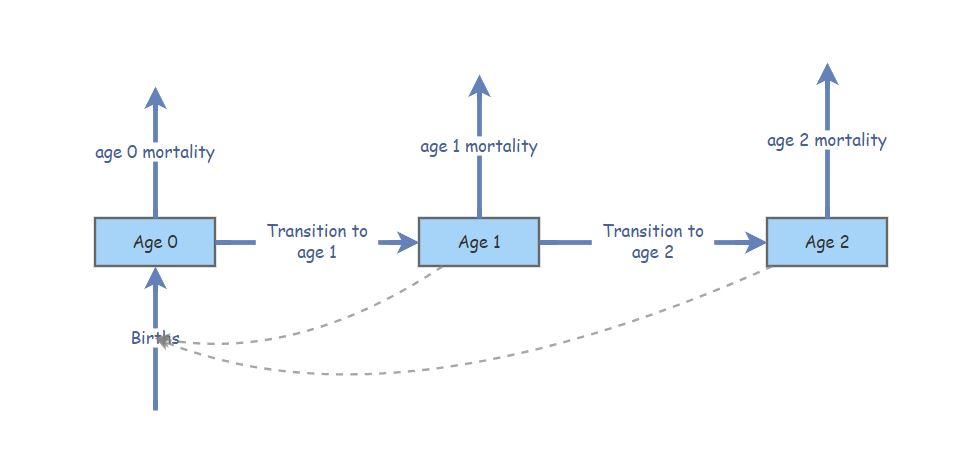
\includegraphics[width=0.5\textwidth,height=\textheight]{IM7.jpg}

Make sure the parameters are at the original values specified in
Exercise 3 of Lab 3 (before altering mortality rates as part of lab 3
question 3c). As a reminder, here they are again:

Age 3 birth rate: 12 (12 female offspring per female, assuming a female
only model)\\
Age 0 survival: 0.1 (10\%)\\
Age 1 survival: 0.9 (90\%)\\
Age 2 survival: 0.5 (50\%)\\
Age 3 survival: 0 (100\% mortality- no individuals survive to age 4)\\
Initial N, Age 1: 100\\
Initial N, Age 2: 100\\
Initial N, Age 3: 50\\
For the mortality rates, note that all individuals in the \emph{Age 1}
stock must either transition to \emph{Age 2} or die. In addition, all
individuals in the \emph{Age 3} stock must die- there is no \emph{Age 4}
class!

Translate this InsightMaker model into a projection matrix with three
rows and three columns. Pay close attention to the difference between
survival (transition to the next stage class) and mortality (mortality
is equal to one minus survival).

2a (image upload). Upload an image file of the full transition matrix (9
numbers, arranged in 3 rows and 3 columns) to WebCampus. To maximize
your chance for partial credit, include all calculations you needed to
arrive at your final solution.

Starting with 75 individuals, all in Age 1 (75 age 1, 0 age 2, 0 age 3),
project this population 20 years into the future, using both
InsightMaker and R.

2b (image upload). Upload an image (plot) of abundance over time for all
ages, produced using R. The x-axis should represent time in years (years
0 to 20), and the y axis should represent abundance. The plot should
include 3 lines, one for each age. (HINT: you can re-use the R code
above to produce this plot).

2c (image upload). Upload an image (plot) of abundance over time for all
ages, produced using InsightMaker. The x-axis should represent time in
years (years 0 to 20), and the y axis should represent abundance. The
plot should include 3 lines, one for each age.

HINT: check your answers to 2b and 2c by comparing the two plots: These
plots should look essentially identical!

Now let's build an InsightMaker model based on a population matrix!

\hypertarget{exercise-3-translate-stage-structured-projection-matrix-to-insightmaker}{%
\subsection{Exercise 3: translate stage-structured projection matrix to
Insightmaker!}\label{exercise-3-translate-stage-structured-projection-matrix-to-insightmaker}}

\hypertarget{use-the-following-stage-matrix-to-answer-questions-3a-b}{%
\paragraph{Use the following stage matrix to answer questions
3a-b}\label{use-the-following-stage-matrix-to-answer-questions-3a-b}}

Here is a stage-based matrix to use for building your InsightMaker
model:

Click \href{stage_matrix1.csv}{here} to download the CSV file.\\
Click \href{stage_matrix1.xlsx}{here} to download the same matrix as an
Excel file.

\begin{Shaded}
\begin{Highlighting}[]
\NormalTok{stmat }\OtherTok{\textless{}{-}} \FunctionTok{read.csv}\NormalTok{(}\StringTok{"stage\_matrix1.csv"}\NormalTok{)}
\NormalTok{stmat }\OtherTok{\textless{}{-}} \FunctionTok{as.matrix}\NormalTok{(stmat[,}\SpecialCharTok{{-}}\DecValTok{1}\NormalTok{])}
\FunctionTok{rownames}\NormalTok{(stmat) }\OtherTok{\textless{}{-}} \FunctionTok{colnames}\NormalTok{(stmat)}
\NormalTok{stmat}
\end{Highlighting}
\end{Shaded}

\begin{verbatim}
##        Stage1 Stage2 Stage3
## Stage1   0.08   0.50   0.82
## Stage2   0.35   0.10   0.00
## Stage3   0.00   0.65   0.80
\end{verbatim}

\begin{Shaded}
\begin{Highlighting}[]
\CommentTok{\# lambda(stmat) }
\end{Highlighting}
\end{Shaded}

Build an InsightMaker model that represents the same population as the
stage-based matrix above. Remember that the top row represents fecundity
terms, while the remaining rows represent transition terms. Also
remember how to convert between survival rates and mortality rates
(mortality equals one minus survival). Initialize the model with 100
individuals at stable stage distribution (SSD).

3a (short answer). Provide the URL to your InsightMaker model (and
remember to clone your Insight to ensure that you don't alter the model
once you submit it).

Next, project this population 20 years into the future using both R AND
InsightMaker.

3b (image upload). Upload an image (plot) of abundance over time for all
ages, produced using R. The x-axis should represent time in years (years
0 to 20), and the y axis should represent abundance. The plot should
include 3 lines, one for each age.

3c (image upload). Upload an image (plot) of abundance over time for all
ages, produced using InsightMaker. The x-axis should represent time in
years (years 0 to 20), and the y axis should represent abundance. The
plot should include 3 lines, one for each age.

HINT: check your answers to 3b and 3c by comparing the two plots: These
plots should look essentially identical!

NOTE: In this class we have stressed the importance of density
dependence in determining and regulating the dynamics of real
populations. Were any of the population models in this lab
density-dependent? {[}Answer: NO! In adding one new type of complexity
to our models- age structure- we have temporarily ``forgotten'' about
density-dependence!{]}

\hypertarget{exercise-4.-translate-written-population-description-to-projection-matrix}{%
\subsection{Exercise 4. Translate written population description to
projection
matrix!}\label{exercise-4.-translate-written-population-description-to-projection-matrix}}

As a test of your understanding, try to build a matrix projection model
based on the following written passage:

\begin{quote}
We assumed that the tawny rat-hawk life history could be described in
terms of four major life stages: juvenile (one-year-olds), subadults
(2-year-olds), non-territorial adults, and territorial adults (all
individuals 3 years old and beyond are considered adults). We assumed
that territorial adult females experienced an average of 10\% mortality
each year, and non-territorial adults experienced 18\% mortality
annually. Juvenile female mortality was 25\% per year, and subadult
mortality was 20\%. Hatchlings (newborns) had a 30\% chance of surviving
their first year of life. We assumed that 90\% of surviving subadults
would become non-territorial adults, while the remaining 10\% would
become territorial adults. We assumed that 45\% of surviving
non-territorial females would successfully transition to the
``territorial adult'' stage, while 10\% of surviving territorial adults
would lose their territories, becoming non-territorial adults.
Territorial adults are the primary reproductive stage, and produce an
average of 2.5 fledged hatchlings each year, half of which are female.
Non-territorial adults produce 1.1 new fledged hatchlings each year on
average, half of which are female. We ran a female-only matrix
population model, and we initialized the population with 800 hatchlings,
150 juveniles, 75 non-territorial adults and 50 territorial adults.
\end{quote}

4a (image upload). Upload an image file of the full transition matrix
(16 numbers, arranged in 4 rows and 4 columns) to WebCampus. To maximize
your chance for partial credit, include all calculations you needed to
arrive at your final solution.

4b (short answer: four numbers). How many juveniles, subadults,
non-territorial adults and territorial adults would there be in the
population at time 0 if you were to initialize the population with 1000
individuals at S.S.D.? (1000 total individuals at time 0).

4c (one number). What is the finite growth rate, Lambda, for this
population?

\#\#Checklist for Lab 4 completion

\begin{itemize}
\item
  Please submit all responses using WebCampus!
\item
  As always, URLs for your InsightMaker models should be pasted in your
  lab submission (in WebCampus). See details below\ldots{}
\end{itemize}

\textbf{\emph{Due Fri Mar.~8 at 11:59pm}}

\begin{itemize}
\tightlist
\item
  Webcampus submission

  \begin{itemize}
  \tightlist
  \item
    \textbf{Exercise 1}

    \begin{itemize}
    \tightlist
    \item
      \emph{image upload (1a.)}\\
    \item
      \emph{short answer (1b.)}\\
    \item
      \emph{short answer (1c.)}
    \item
      \emph{short answer (1d.)}
    \item
      \emph{short answer (1e.)}
    \item
      \emph{short answer (1f.)}
    \item
      \emph{short answer (1g.)}
    \item
      \emph{short answer (1h.)}
    \item
      \emph{image upload (1i.)}
    \end{itemize}
  \item
    \textbf{Exercise 2}

    \begin{itemize}
    \tightlist
    \item
      \emph{image upload (2a.)}
    \item
      \emph{image upload (2b.)}
    \item
      \emph{image upload (2c.)}
    \end{itemize}
  \item
    \textbf{Exercise 3}

    \begin{itemize}
    \tightlist
    \item
      \emph{short answer (3a.)}
    \item
      \emph{image upload (3b.)}
    \item
      \emph{image upload (3c.)}
    \end{itemize}
  \item
    \textbf{Exercise 4}

    \begin{itemize}
    \tightlist
    \item
      \emph{image upload (4a.)}
    \item
      \emph{short answer (4b.)}
    \item
      \emph{short answer (4c.)}
    \end{itemize}
  \end{itemize}
\end{itemize}

---End of Lab 4----

\end{document}
